\documentclass{beamer}
\usepackage{times, amsthm, amsmath, amssymb, cancel, changepage, graphicx, lipsum, fancyhdr, mathabx, enumitem,caption, subcaption}
\usetheme{CambridgeUS}
\usecolortheme{seagull}
\usefonttheme{serif}
\definecolor{navy}{RGB}{0, 0, 128} 
\setbeamercolor{frametitle}{fg=navy}
\setbeamercolor{title}{fg=navy}

\title{\textbf{Lecture 3: Integration Fundamentals}}
\date{September 3, 2019}

\begin{document}
	
\frame{\titlepage}

\begin{frame}
\frametitle{\textbf{Intro to Integration}}

\begin{figure}
	\centering
	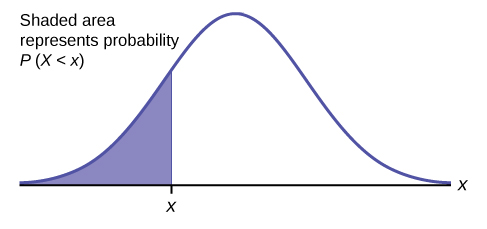
\includegraphics[height=.4\textheight]{normal-dist.jpg}\\
	\hspace*{10pt}\hbox{\thinspace{\tiny\itshape Lumen Learning}}
\end{figure}

Integration is a technique to find the area under a curve $f(x)$ over some interval $[a,b]$. In statistics, we use this often to find probabilities like $P(X<x)$ for some random variable $X$.

\end{frame}

\begin{frame}
\frametitle{\textbf{Riemann Integration: Basic Idea}}

\begin{figure}
	\centering
	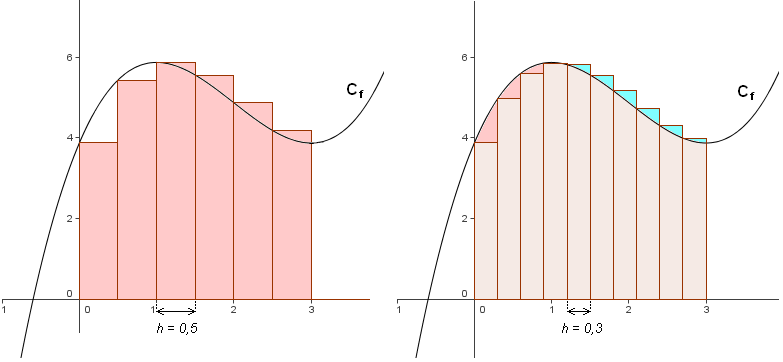
\includegraphics[height=.4\textheight]{subintervals.png}\\
	\hspace*{10pt}\hbox{\thinspace{\tiny\itshape Science Direct}}
\end{figure}

Riemann integration involves using smaller and smaller rectangles to find the area under $f(x)$. As the width of these rectangles goes to zero, the approximation of the area becomes more and more accurate.
\end{frame}


\begin{frame}
\frametitle{\textbf{Approximating the Area Under $F(x)$}}
Goal: find the area $S$ under $f(x)$ over some interval $I=[a,b]$.
\begin{itemize}
	\item[1.] Divide $I$ into $n$ smaller subintervals by choosing points $a=x_0<x_1<...<x_n=b$
	\item[2.] The $n$ subintervals are then $[x_0,x_1],[x_1,x_2],...,[x_{n-1},x_n]$. This is called the partition of $I$ and is denoted by $\mathbb{P}$
	\item[3.] Define $\Delta x_i = x_i-x_{i-1}$.
	\item[4.] The length of the longest subinterval is given by the norm $||\mathbb{P}|| = \max\{\Delta x_1,...,\Delta x_n\}$
	\item[5.] Divide $S$ into strips $s_1,...,s_n$ by drawing the vertical lines at $x_0,x_1,...,x_n$
	\item[6.] Choose an $x_i^*$ in each subinterval and construct a rectangle $R_i$ with base $\Delta x_i$ and height $f(x_i^*)$.
	\item[7.] Define $A_i = f(x_i^*) \Delta x_i$ as the area of $R_i$.
	\item[8.] Then $\sum_{i=1}^{n} A_i = \mbox{ area of } S$
	\item[9.] $A = \lim\limits_{||\mathbb{P}|| \to 0} \sum_{i=1}^{n} A_i$
\end{itemize}


\end{frame}

\begin{frame}
\frametitle{\textbf{Definite Integral}}
If $f$ is a function defined on a closed interval $[a,b]$, let $\mathbb{P}$ be a partition of $[a,b]$ with points $x_0,...,x_1$ where $a=x_0<x_1<...<x_n=b$. Choose points $x_i^*$ in $[x_{i-1},x_i]$ and let $\Delta x_i = x_i - x_{i-1}$ and $||\mathbb{P}|| = \max\{ \Delta x_i \}$. Then the definite integral of $f$ from $a$ to $b$ is given by

$$\int_{a}^{b} f(x)dx =  \lim\limits_{||\mathbb{P}|| \to 0} \sum_{i=1}^{n} \Delta x_i \, f(x_i^*)$$

if this limit exists. If it does exists $f$ is integrable on $[a,b]$.\\

\vspace{6pt}
\textit{Note: $f$ is integrable on $[a,b]$ if it is continuous on $(a,b)$.}

\vspace{6pt}
\textbf{Example:}
\begin{itemize}
	\item[(a)] Estimate the area of the region between the x-axis and $f(x) = x^3-2x^2+4$ using the left, right, and midpoint of subintervals for the height of $n=5$ rectangles.
\end{itemize}

\end{frame}

\begin{frame}
\frametitle{\textbf{Properties of the Definite Integral}}
Let $c \in \mathbb{R}$ and let $f(x),g(x)$ be continuous functions on the closed interval $[a,b]$. Then the following properties hold:
\begin{itemize}
	\item[1.] $\int_{a}^{b} c \mathop{dx} = c(b-a)$
	\item[2.] $\int_{a}^{b} [f(x) + g(x)] \mathop{dx} = \int_{a}^{b} f(x) \mathop{dx} + \int_{a}^{b} g(x) \mathop{dx}$
	\item[3.] $\int_{a}^{b}c f(x) \mathop{dx} = c\int_{a}^{b} f(x) \mathop{dx} $
	\item[4.] $\int_{a}^{b} f(x) \mathop{dx} \leq \int_{a}^{b} g(x) \mathop{dx} $ if $f(x) \leq g(x) \, \forall x \in [a,b]$
	\item[5.] $\int_{a}^{b} f(x) \mathop{dx} = \int_{a}^{c} f(x) \mathop{dx} + \int_{c}^{b} f(x) \mathop{dx}$ for $c \in [a,b]$
	\item[6.] $\int_{a}^{a} f(x) \mathop{dx} =0$
	\item[7.] $\int_{a}^{b} f(x) \mathop{dx} = - \int_{b}^{a} f(x) \mathop{dx} $
	\item[8.] $\Big| \int_{a}^{b} f(x) \mathop{dx} \Big| \leq \int_{a}^{b} |f(x)| \mathop{dx} $
\end{itemize}
\end{frame}




\begin{frame}
\frametitle{\textbf{Fundamental Theorem of Calculus}}

\begin{theorem}[Fundamental Theorem of Calculus]
	If $f$ is continuous on $[a,b]$ and the function $F$ is defined by
	$$ F(x) = \int_{a}^{x} f(t) \mathop{dt}$$
	then $F$ is an anti-derivative of $f$ on $[a,b]$ and $F'(x) = f(x)$. Furthermore, if $F$ is any anti-derivative of $f$ then
	$$ \int_{a}^{b} f(x) \mathop{dx} = F(x) \Big|_a^b = F(b) - F(a)$$
\end{theorem}

\vspace{6pt}

A list of common anti-derivatives can be found \href{https://www.wyzant.com/resources/lessons/math/calculus/integration/antiderivatives}{\beamergotobutton{Here}}.
\end{frame}


\begin{frame}
\frametitle{\textbf{Some Examples Using Definite Integrals}}

\begin{itemize}
	\item[(a)] Determine the value of $\int_{2}^{9}f(x) \mathop{dx}$ given that  $\int_{5}^{92}f(x) \mathop{dx} = 3$ and  $\int_{5}^{9}f(x) \mathop{dx} = 8$.
	\item[(b)] $\int_{a}^{b}3x^4 + 6x^2 + 2 \mathop{dx}$
	\item[(c)] $\int_{a}^{b} 7e^x + \frac{2}{x} \mathop{dx}$
	\item[(d)] $\int_{0}^{4} f(x) \mathop{dx}$ where $f(x) = \begin{cases}
	2x & x>1\\ 1-3x^2 & x \leq 1
	\end{cases}$
	\item[(d)] $\int_3^6 |2x-10| \mathop{dx}$
\end{itemize}
\end{frame}

\begin{frame}
\frametitle{\textbf{Indefinite Integrals}}
A definite integral has a specified interval $[a,b]$ while an indefinite integral has unspecified interval.
$$\int f(x) \mathop{dx} = F(x) + C$$

\vspace{6pt}
\textbf{Examples:}
\begin{itemize}
	\item[(a)] $\int \sqrt[3]{x} + 10 \sqrt[5]{x^3} \mathop{dx}$
	\item[(b)] $\int \frac{2}{\theta}e^{-\frac{2}{\theta}} \mathop{dx}$
	\item[(c)] Determine $f(x)$ given that $f'(x) = 12x^2-4x$ and $f(-3)=17$
\end{itemize}
\end{frame}

%\begin{frame}
%\frametitle{What is a Limit?}
%\begin{figure}
%	\centering
%	\begin{subfigure}{0.48\textwidth}
%		
%		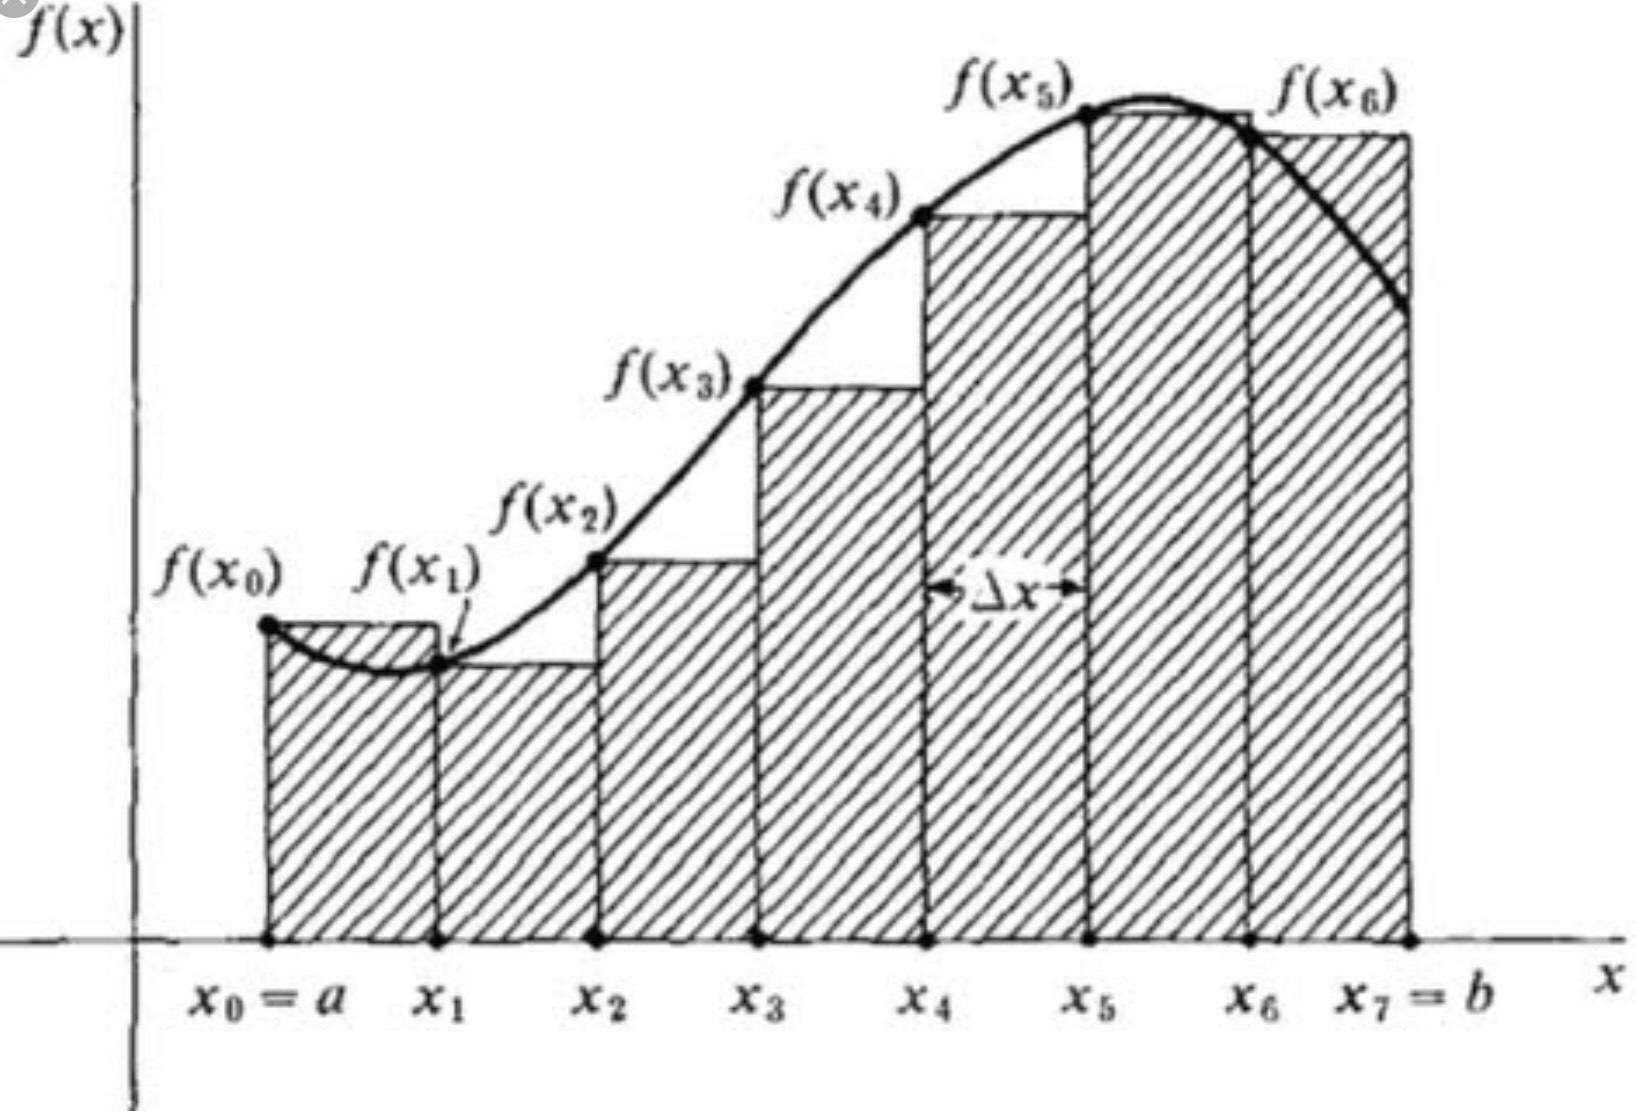
\includegraphics[width=\textwidth]{IMG_0380.jpg}
%		\hspace*{10pt}\hbox{\thinspace{\tiny\itshape vias.org}}
%		\caption{Single integration}
%	\end{subfigure}% 
%	~ 
%	\begin{subfigure}{0.48\textwidth}
%		
%		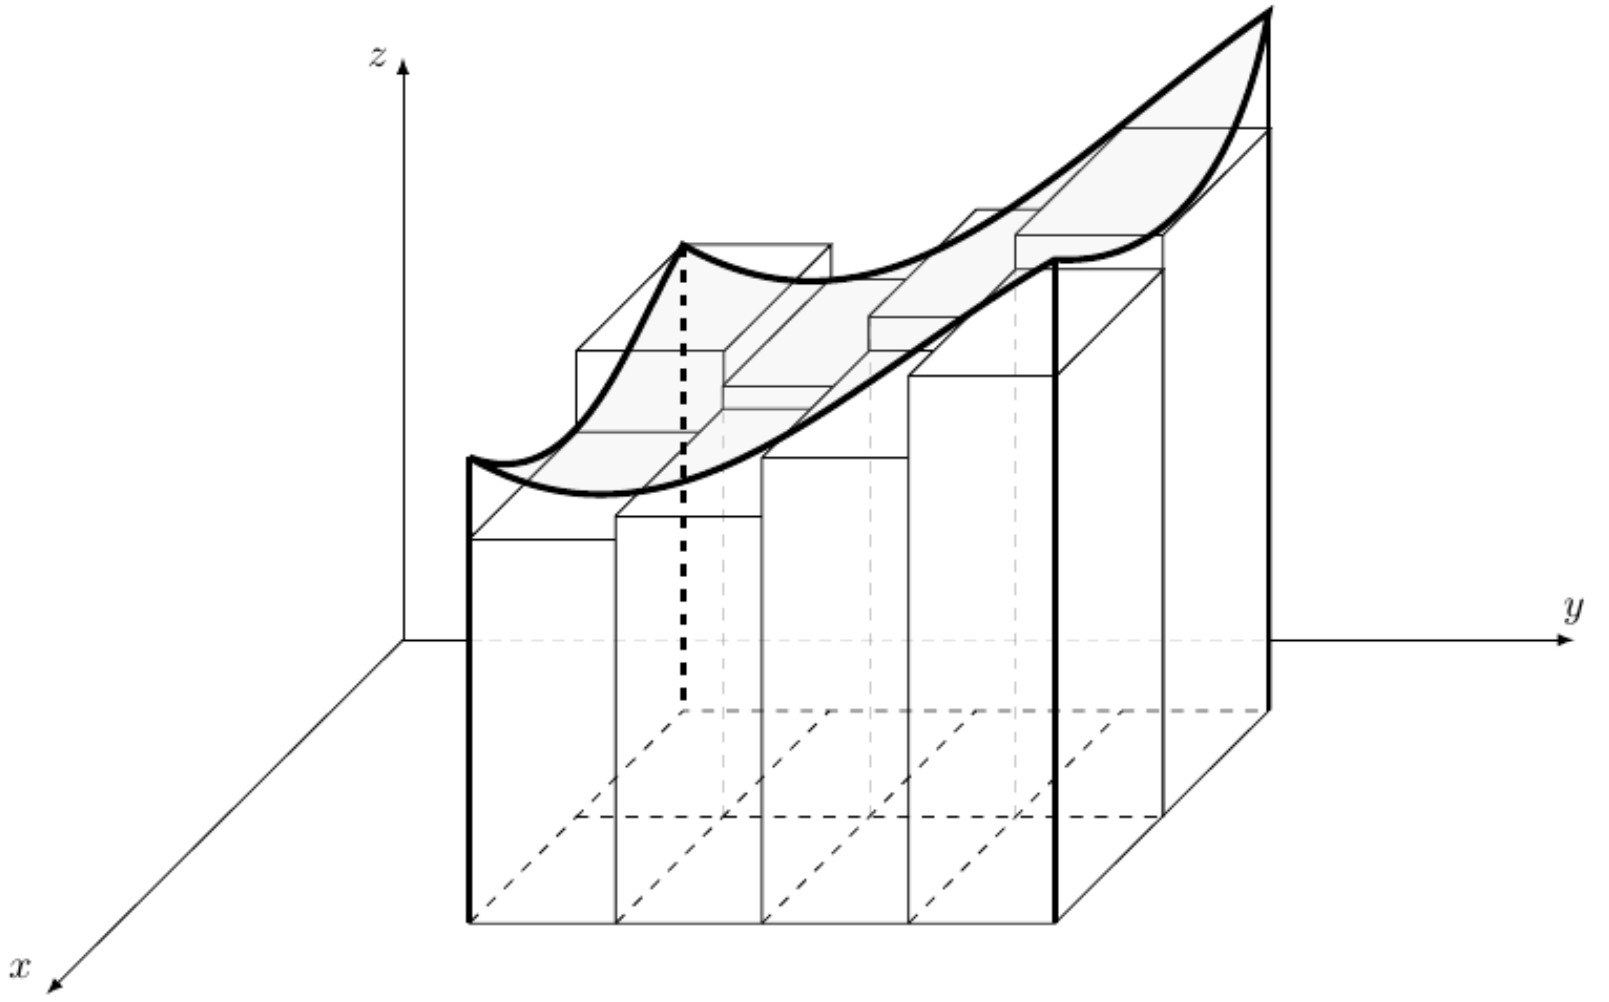
\includegraphics[width=\textwidth]{IMG_0385.jpg}
%		\hspace*{10pt}\hbox{\thinspace{\tiny\itshape tex.stackexchange.com}}
%		\caption{Double integration.}
%		\label{fig:2}
%	\end{subfigure}
%\end{figure}
%
%\end{frame}
%
%
%\begin{frame}
%\frametitle{Triple Integral}
%\begin{figure}
%	\centering
%	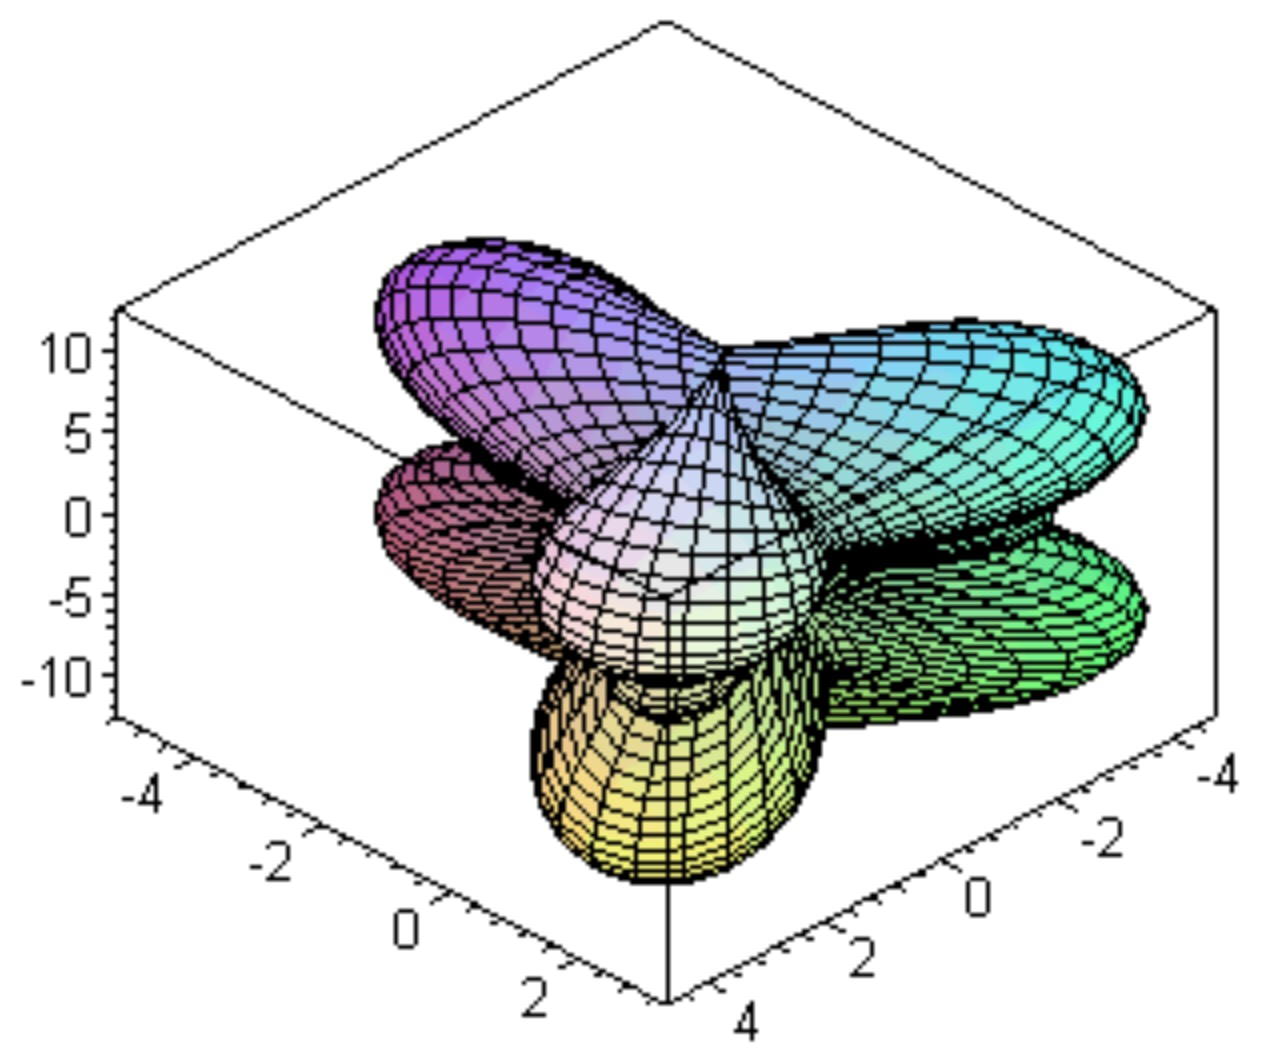
\includegraphics[height=.45\textheight]{IMG_0384.jpg}\\
%	\hspace*{10pt}\hbox{\thinspace{\tiny\itshape maplesoft.com}}
%\end{figure}
%
%$$\iiint\limits_{\mathbb{R}} F(x,y,z) dV = \int_{x=a}^{x=b} \int_{y=y_1(x)}^{y=y_2(x)} \int_{z=z_1(x,y)}^{z=z_2(x,y)} F(x,y,z) dz\,dy\,dx$$
%\textbf{Example:}
%\begin{itemize}
%	\item[(a)] $\int_0^1 \int_0^{1-x} \int_0^{2-x} xyz \,dz\,dy\,dx$
%\end{itemize}
%\end{frame}

\end{document}
